\section{Simulador de radiología diagnóstica}
\label{result:xray}

%Para demostrar las capacidades del algoritmo propuesto de adaptar la posición de un paciente virtual con tasas de refresco interactivas, se desarrolló un simulador de radiología diagnóstica. 
El simulador de radiología diagnóstica desarrollado ofrece una plataforma de enseñanza y autoprendizaje para practicar las proyecciones radiológicas, donde el usuario puede cambiar la postura del paciente virtual y visualizar su radiografía de manera interactiva. 

En la figura \ref{fig:simui} se puede observar la \ac{IU} del simulador. En esta imagen se puede observar las funcionalidades del simulador citadas en la sección \ref{xray:courseware}. 
%En la zona central, se encuentra la vista de la escena 3D. En esta ventana, se podrá observar el modelo virtual cargado para la ocasión situado en una sala de radiología virtual. El usuario podrá utilizar el ratón para mover la perspectiva de la cámara y hacerse una idea de la escena virtual.
%En la esquina superior izquierda se sitúa el módulo de posicionamiento del modelo virtual. En esta división, el usuario puede seleccionar posturas previamente guardadas o almacenar nuevas posiciones. Además, puede seleccionar de manera individual cada articulación que disponga el modelo virtual. 
\begin{figure}[h]
\centering
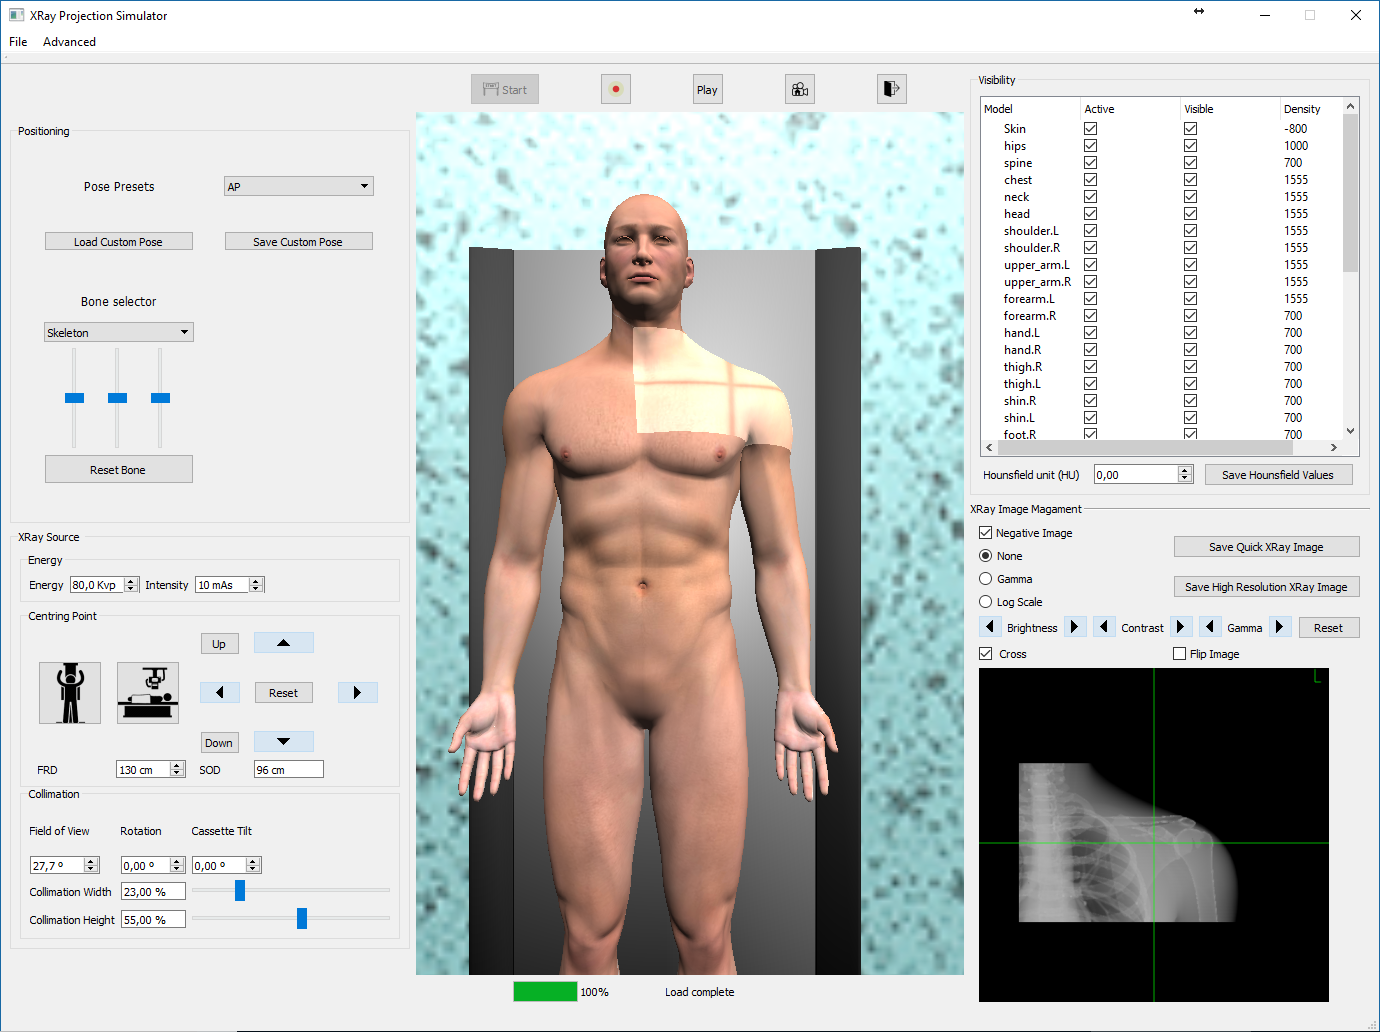
\includegraphics[width=0.95\linewidth]{IMG/simui.png}
\caption{\label{fig:simui} Interfaz de usuario del simulador de radiología diagnóstica. }
\end{figure}

%En la esquina inferior izquierda, se puede observar todos los parámetros relacionados con la configuración del emisor de rayos X con el objetivo de conseguir una imagen radiográfica de calidad.
%Por otra parte, en la esquina superior derecha se encuentra una lista de los tejidos del paciente virtual que están disponibles. En esta lista, se puede esconder los tejidos bajo demanda o se puede cambiar sus propiedades químicas. Esta funcionalidad permite al usuario comprobar multitud de variaciones del modelo virtual cargado.

%Por último, en la esquina inferior derecha se puede observar la imagen de rayos X resultante de la posición del emisor en relación con el modelo virtual. En esta imagen se podrá apreciar la configuración de la colimación o de los distintos parámetros que definen un emisor de rayos X. Además, la imagen resultante puede ser modificada en cuanto a brillo, contraste, o filtros de imágenes. Esto ayuda al usuario a interpretar y entender la imagen al ocultar o resaltar detalles de la anatomía.

\subsection{Rendimiento}
En cuanto al rendimiento de la aplicación, ambos algoritmos (posicionador de pacientes virtuales y la librería de simulación de rayos X) se ejecutan interactivamente. En el peor de los casos, el modelo de \emph{ZygoteBody}$^{TM}$ y su malla de tetraedros se componen de 1.5 millones de vértices y 2.5 millones de tetraedros. El simulador es capaz de mantenerse por encima de las 25 imágenes por segundo. \todo{medir tiempos en el despacho}

\begin{table}[h]
\centering
\caption{Tiempo en milisegundos de los dos módulos que componen el simulador. ZM es Zygote Masculino, ZF es Zygote Femenino, A es Anatomium }
\begin{tabular}{|c|c|c|}
%\multirow{2}{*}{\textbf{Model}} & \multicolumn{2}{c}{\textbf{Interactive stage}} & \multirow{2}{*}{\textbf{Optimization}} \\
\hline
\textbf{Modelo}&\textbf{TPTVPH} &\textbf{gVirtualXRay}  \\ 
\hline
ZM  & 25-16 & 22-18 \\ 
\hline
ZF  & 29-21  & 23-17    \\ 
\hline
A   & 20-13 & 21-18 \\ 
\hline
HVP   & 17-08 & 15-12 \\ 
\hline
\end{tabular}
\label{tab:xraytime}
\end{table}

%Para alcanzar estas tasas de refresco, el algoritmo propuesto delega las operaciones más complejas a un proceso previo descrito en la sección \ref{posing:result}.
%El mayor consumo de tiempo viene dado por el proceso previo del algoritmo propuesto (ver sección \ref{posing:result}) y la complejidad del modelo virtual, que en el caso de \emph{ZygoteBody}$^{TM}$ toma menos de 7 minutos.


\subsection{Resultados visuales}

Los modelos anatómicos presentados en la sección \ref{posing:result} se han utilizado como modelos de entrada en el simulador. En esta herramienta, se puede incorporar cualquier modelo anatómico externo, utilizando el preproceso previo de la herramienta \ac{TPTVPH}. Se han utilizado los modelos presentados en \ref{fig:models}. En la figura \ref{fig:xraymodels} se muestran los cuatro modelos completos y su correspondiente radiografía de pecho.

\begin{figure}[h]
    \begin{subfigure}[b]{0.24\linewidth}
        \centering
        {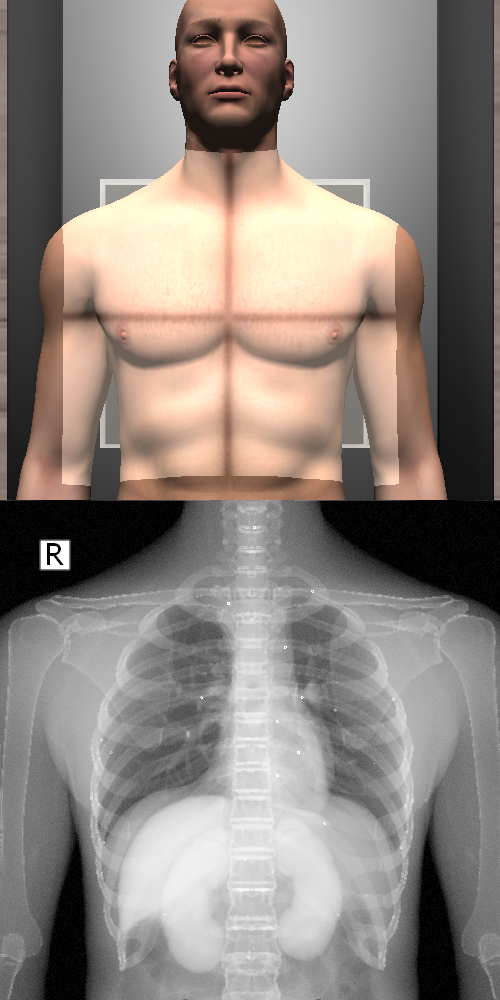
\includegraphics[width=\linewidth]{IMG/zygoteex.png}}
        \caption{\emph{ZygoteBody}$^{TM}$ Masculino.}
    \end{subfigure}
     \begin{subfigure}[b]{0.24\linewidth}
        \centering
        {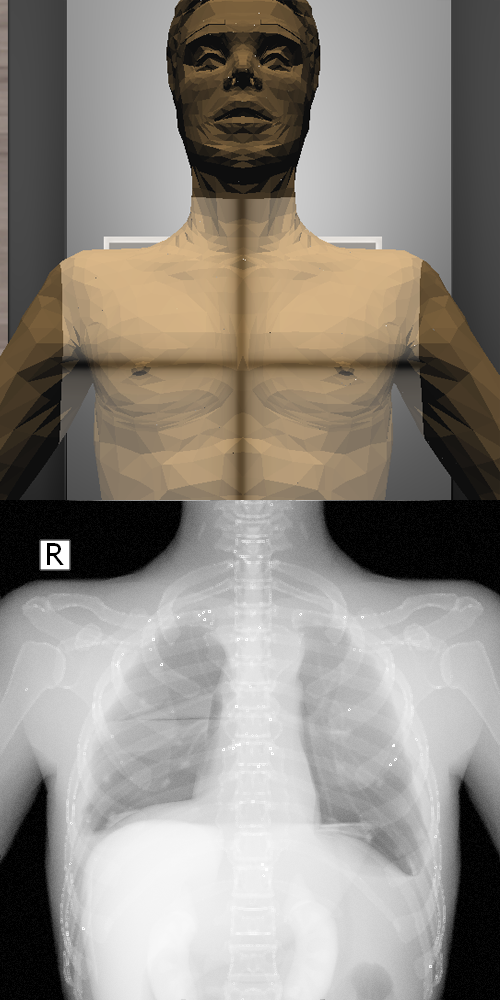
\includegraphics[width=\linewidth]{IMG/anaex.png}}
        \caption{\emph{Anatomium} Masculino.}
    \end{subfigure}
    \begin{subfigure}[b]{0.24\linewidth}
        \centering
        {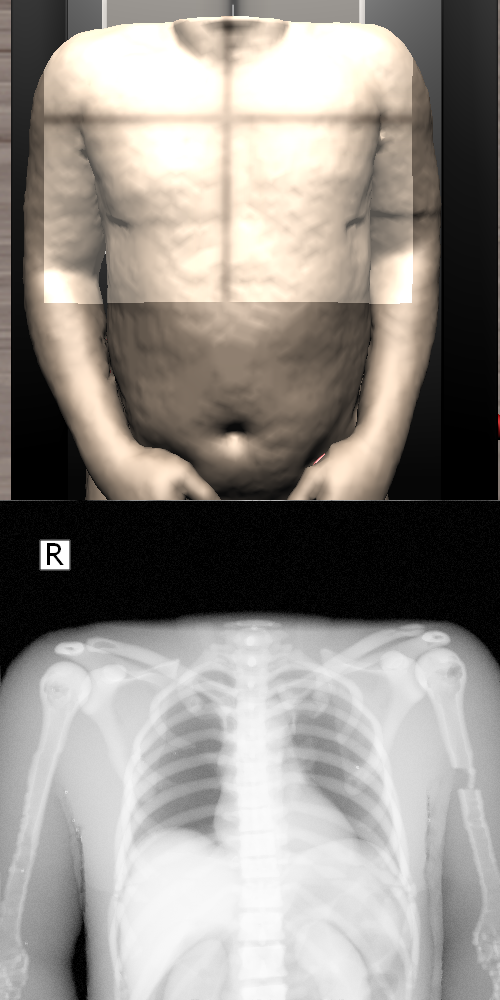
\includegraphics[width=\linewidth]{IMG/HVPex.png}}
        \caption{\emph{Segmented Inner Organs}\label{subfig:HVP}.}
    \end{subfigure}
     \begin{subfigure}[b]{0.24\linewidth}
        \centering
        {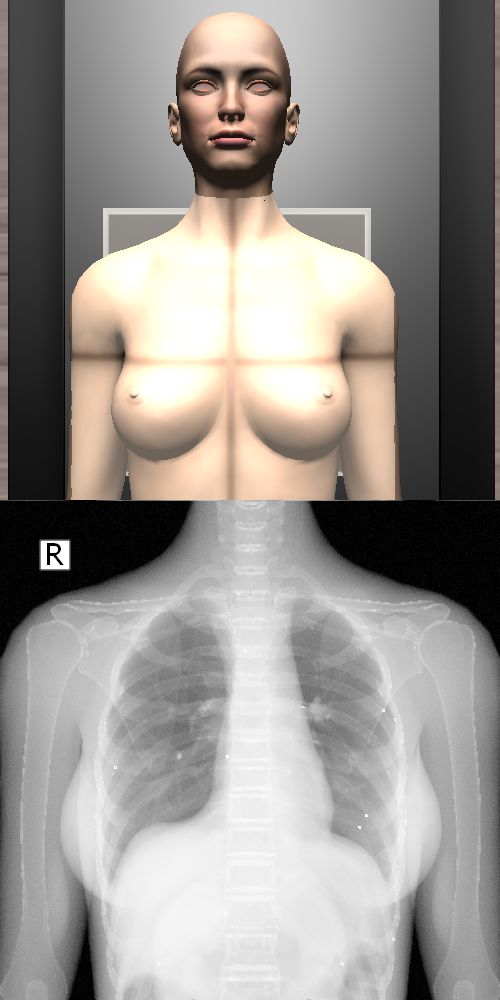
\includegraphics[width=\linewidth]{IMG/femaleex.png}}
        \caption{\emph{ZygoteBody}$^{TM}$ Femenino.}
    \end{subfigure}
    \caption{\label{fig:xraymodels} Modelos utilizados en el simulador de radiología diagnóstica.}
   \end{figure}
   
Como se puede observar, la calidad de la imagen radiográfica depende de la calidad del modelo del paciente virtual. %En concreto, los modelos comerciales necesitan una pequeña adaptación en los tejido óseos para mejorar el realismo de las imágenes. Los huesos presentan dos tipos de tejidos: 
% \begin{itemize}
%     \item Cortical: tejido denso que se encuentra en la capa externa de los huesos.
%     \item Trabecular: capa esponjosa que se encuentra en el interior de los huesos.
% \end{itemize}
Es habitual, que los modelos comerciales proporcionan una representación solamente superficial de los huesos (cortical \footnote{tejido denso que se encuentra en la capa externa de los huesos.}) y suelen ignorar los tejidos internos (trabecular\footnote{capa esponjosa que se encuentra en el interior de los huesos}). Sin embargo, la librería \emph{gVirtualXRay} se basa en la funcionalidad de trazador de rayos. Se calcula el recorrido del rayo a través de las estructuras anatómicas, entrando por la cara frontal del triángulo y salir por la cara trasera de otro triángulo de la misma malla. Este recorrido sirve para calcular la atenuación del rayo dependiendo de las propiedades físicas del material y la longitud del recorrido. Como consecuencia de la ausencia de los tejidos internos, su representación en la imagen de rayos X parece homogénea en toda su estructura, dando lugar a una imagen no realista (ver fig.~\ref{subfig:nointernal}). Con el objetivo de mejorar la representación de las zonas trabeculares, se ha ha desarrollado una pequeña modificación. Se duplica la superficie del hueso, se invierten las normales, encogiendo la geometría en esa dirección. De esta manera, se crea una estructura interna con una forma similar al hueso. En la figura ~\ref{fig:bonecompare} se puede observar la diferencia entre el modelo original y los tejidos modificados incluyendo las zonas trabeculares. Este problema no ocurre cuando los modelos anatómicos son obtenidos de técnicas como \ac{TC} donde ambos tejidos son fácilmente identificados. El caso del  
\emph{Segmented Inner Organs}\cite{VoxelMan} se puede observar en la figura \ref{subfig:HVP}.




\begin{figure}[h]
    \begin{subfigure}[b]{0.45\linewidth}
        \centering
        {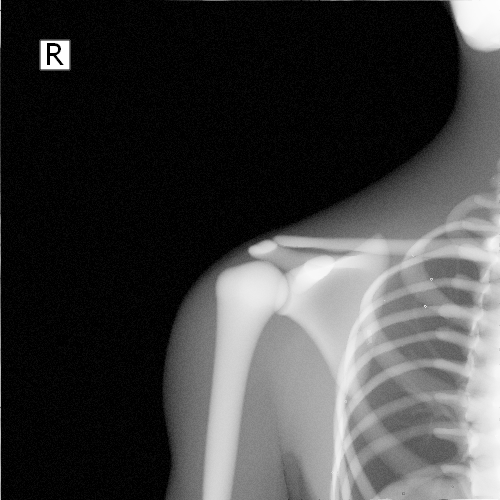
\includegraphics[width=\linewidth]{IMG/xraynointernal.png}}
        \caption{Tejido óseo original del \emph{ZygoteBody}$^{TM}$ Masculino\label{subfig:nointernal}.}
    \end{subfigure}
    \null\hfill
     \begin{subfigure}[b]{0.45\linewidth}
        \centering
        {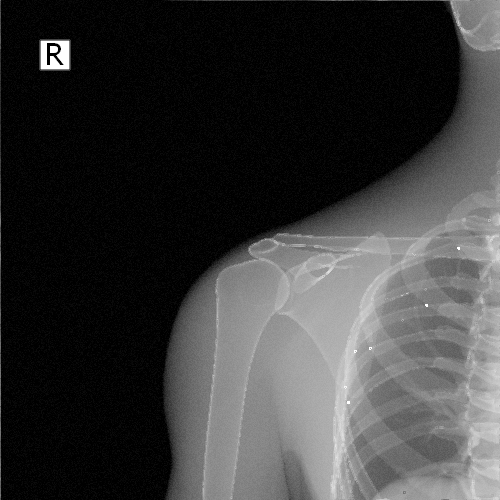
\includegraphics[width=\linewidth]{IMG/xrayinternal.png}}
        \caption{Resultado de la inclusión del tejido interior de los huesos.}
    \end{subfigure}
    \caption{\label{fig:bonecompare} Comparativa entre una el mallado original de \emph{ZygoteBody}$^{TM}$ Masculino y la introducción del tejido trabecular en los huesos.}
   \end{figure}



A continuación, se procederá a mostrar algunos resultados y comparaciones entre la aplicación desarrollada y un libro tradicional de proyecciones radiológicas.
Como se puede observar en la figura \ref{fig:xraycomp}, se han seleccionado unas imágenes de proyecciones radiológicas procedentes del libro \cite{carver2012medical} y se ha procedido a replicar la misma posición en la herramienta. La ventaja de usar la aplicación es que se pueden obtener más imágenes de la misma anatomía o proyección que permitirá a profesores y estudiantes practicar de manera más extensa. 


% \begin{figure}[tb]
% \centering
% 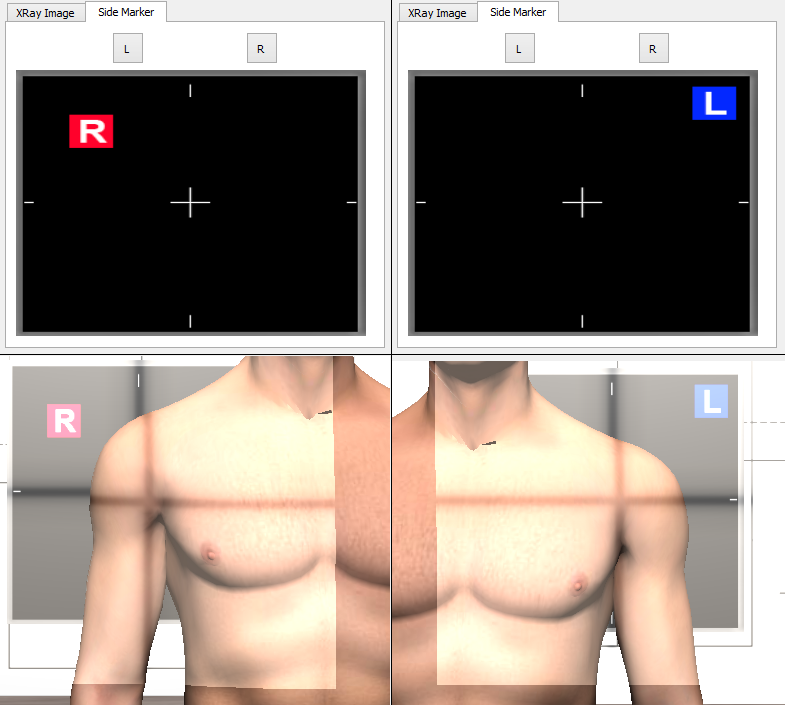
\includegraphics[width=0.5\linewidth]{IMG/side.png}
% \caption{\label{fig:xraycomp} Comparativa entre una imagen del libro\cite{carver2012medical} y la imagen resultante de la herramienta. }
% \end{figure}

\begin{figure}[h]
    \begin{subfigure}[b]{0.45\linewidth}
        \centering
        {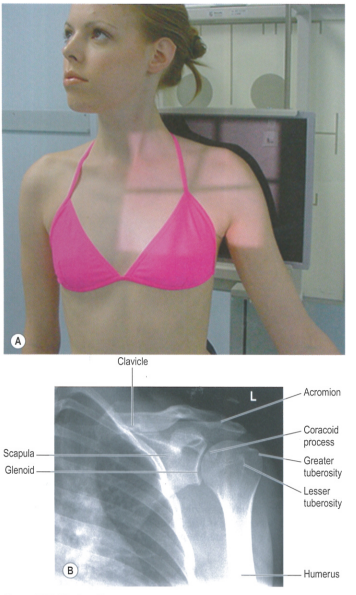
\includegraphics[width=\linewidth]{IMG/carvershoulder.PNG}}
        \caption{Imagen cortesía de E. Carver, B. Carver y Elsevier Health Sciences~\cite{carver2012medical}.}
    \end{subfigure}
    \null\hfill
     \begin{subfigure}[b]{0.45\linewidth}
        \centering
        {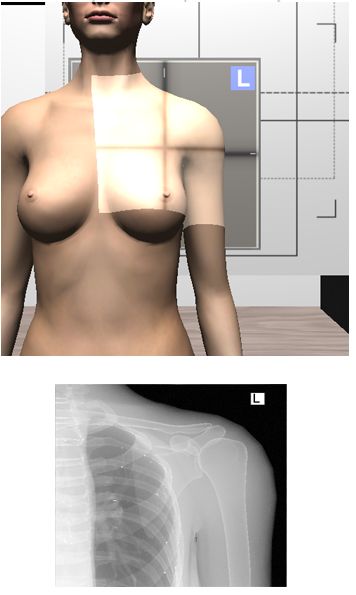
\includegraphics[width=\linewidth]{IMG/XRayshoulder3.png}}
        \caption{Proyección anteroposterior del hombro replicada en el simulador.}
    \end{subfigure}
    \caption{\label{fig:xraycomp} Comparativa entre una imagen del libro\cite{carver2012medical} y la imagen resultante del simulador.}
   \end{figure}

Otra muestra de las ventajas del simulador frente a los materiales educativos tradicionales se puede observar en la figura \ref{fig:disease}. En esta ocasión, es posible generar variaciones anatómicas del mismo modelo. Con ello se pueden enseñar como podría verse una enfermedad y ayudar a la interpretación la imagen. Cambiando unos pocos parámetros, el simulador permite cambiar entre un tejido sano o enfermo. Incluso puede ser interesante que los estudiantes puedan observar como objetos extraños se pueden distinguir cuando se encuentran dentro de la anatomía del paciente. 

% \begin{figure}[tb]
% \centering
% 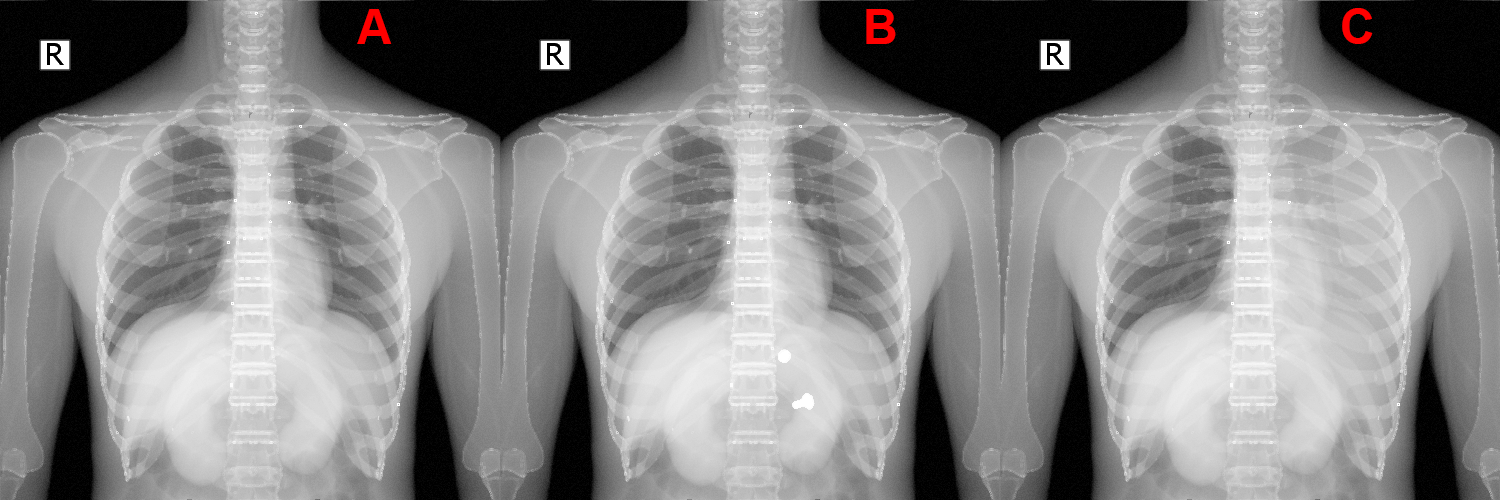
\includegraphics[width=0.5\linewidth]{IMG/disease.png}
% \caption{\label{fig:resultdisease}Usuarios pueden probar diferentes casos. A: Anatomía normal. B: Objetos extraños en el estómago. C: Pulmón izquierdo colapsado. }
% \end{figure}

\subsection{Validación}

Se ha diseñado un estudio para comprobar la validez aparente y contenido del simulador. Se ha pedido a los participantes observar una serie de vídeos que describían las funcionalidades del simulador. A continuación, se le hacía unas preguntas referentes al vídeo y al simulador. Se ha seleccionado como  población objetivo el conjunto de especialistas relacionados con la técnica de radiología. Se buscaba contar con la opinión de estudiantes y profesionales incluyendo varios países. La encuesta se puede consultar en el anexo \ref{anexo:cuestionarioxray}.

Al finalizar la encuesta, se han registrado 18 participaciones (con un $50\%$ de mujeres y hombres): 16 de ellos se han definido como técnico en radiología; de 4 países diferentes ( 15 de Reino Unido, 1 de Francia, 1 de Canadá y 1 de España); con años de práctica de radiología entre 1 y 40 años (ver figura \ref{fig:year}.

En el formulario, se incluía una pregunta sobre la confianza del participante a la hora de tomar una imagen de rayos X. Tal y como se ve en la figura \ref{fig:confident}, muestra un amplio número de participantes que reflejan una alta confianza en sus habilidades.

Por otra parte, también se incluía la pregunta sobre la confianza del participante en sus habilidades para interpretar la radiografía con fines de diagnóstico médico. En la figura \ref{fig:interpreting} se muestra el histograma con los resultados. En este caso, hay más variabilidad en las respuestas.


\begin{figure}[h]
        \centering
        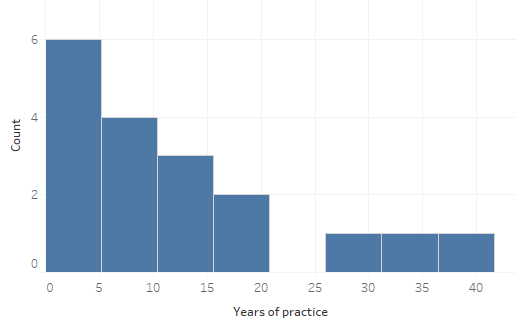
\includegraphics[width=0.75\linewidth]{IMG/years.png}
        {
         \caption{\label{fig:year}Histograma de los años de experiencia de los participantes.}
        }
       
    \end{figure}
     \begin{figure}[h]
        \centering
        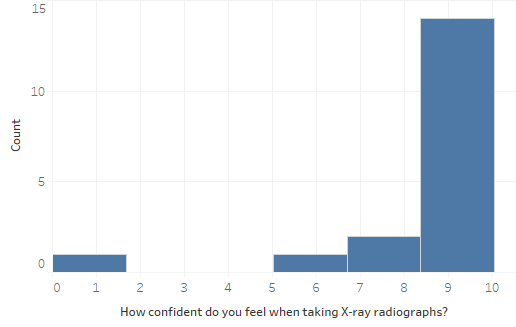
\includegraphics[width=0.75\linewidth]{IMG/confident.png}{
        
        \caption{\label{fig:confident}Histograma de las respuestas a la pregunta sobre como de confiados se sienten al tomar una radiografía.}
        }
    \end{figure}
   
     \begin{figure}[h]
        \centering
        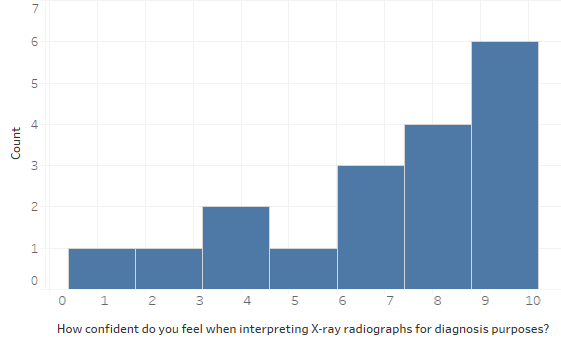
\includegraphics[width=0.75\linewidth]{IMG/interpreting.png}{
        \caption{\label{fig:interpreting}Histograma de las respuestas a la pregunta sobre como de confiados se sienten al interpretar una radiografía con fines diagnóstico.}
        }
    \end{figure}


\subsubsection{Validez aparente}

En cuanto a la validez aparente, se han incluido en la encuesta las preguntas de la tabla \ref{tab:facevalidity}. Estas preguntas eran de tipo \emph{Likert}, donde se podía responder desde 1(Nada de acuerdo) hasta 5(Muy de acuerdo). 

En la figura \ref{fig:facevalidity}, se pueden observar los resultados por cada pregunta mostrados en porcentaje de respuestas. Es destacable que en general hay al menos un 60\% de respuestas positivas en todas las preguntas y ninguna respuesta completamente negativa, excepto la pregunta F3. Esta pregunta trataba sobre la descripción de los pasos que debe realizar un médico cuando esta realizando el procedimiento. Cuando en la sección \ref{art:xraysim} se describió los pasos del procedimiento de proyecciones radiológicas, en el propio libro \cite{manualpractico} se advertía sobre las posibles variaciones dependiendo del lugar de trabajo.  



\begin{figure}[hb]
    \centering
    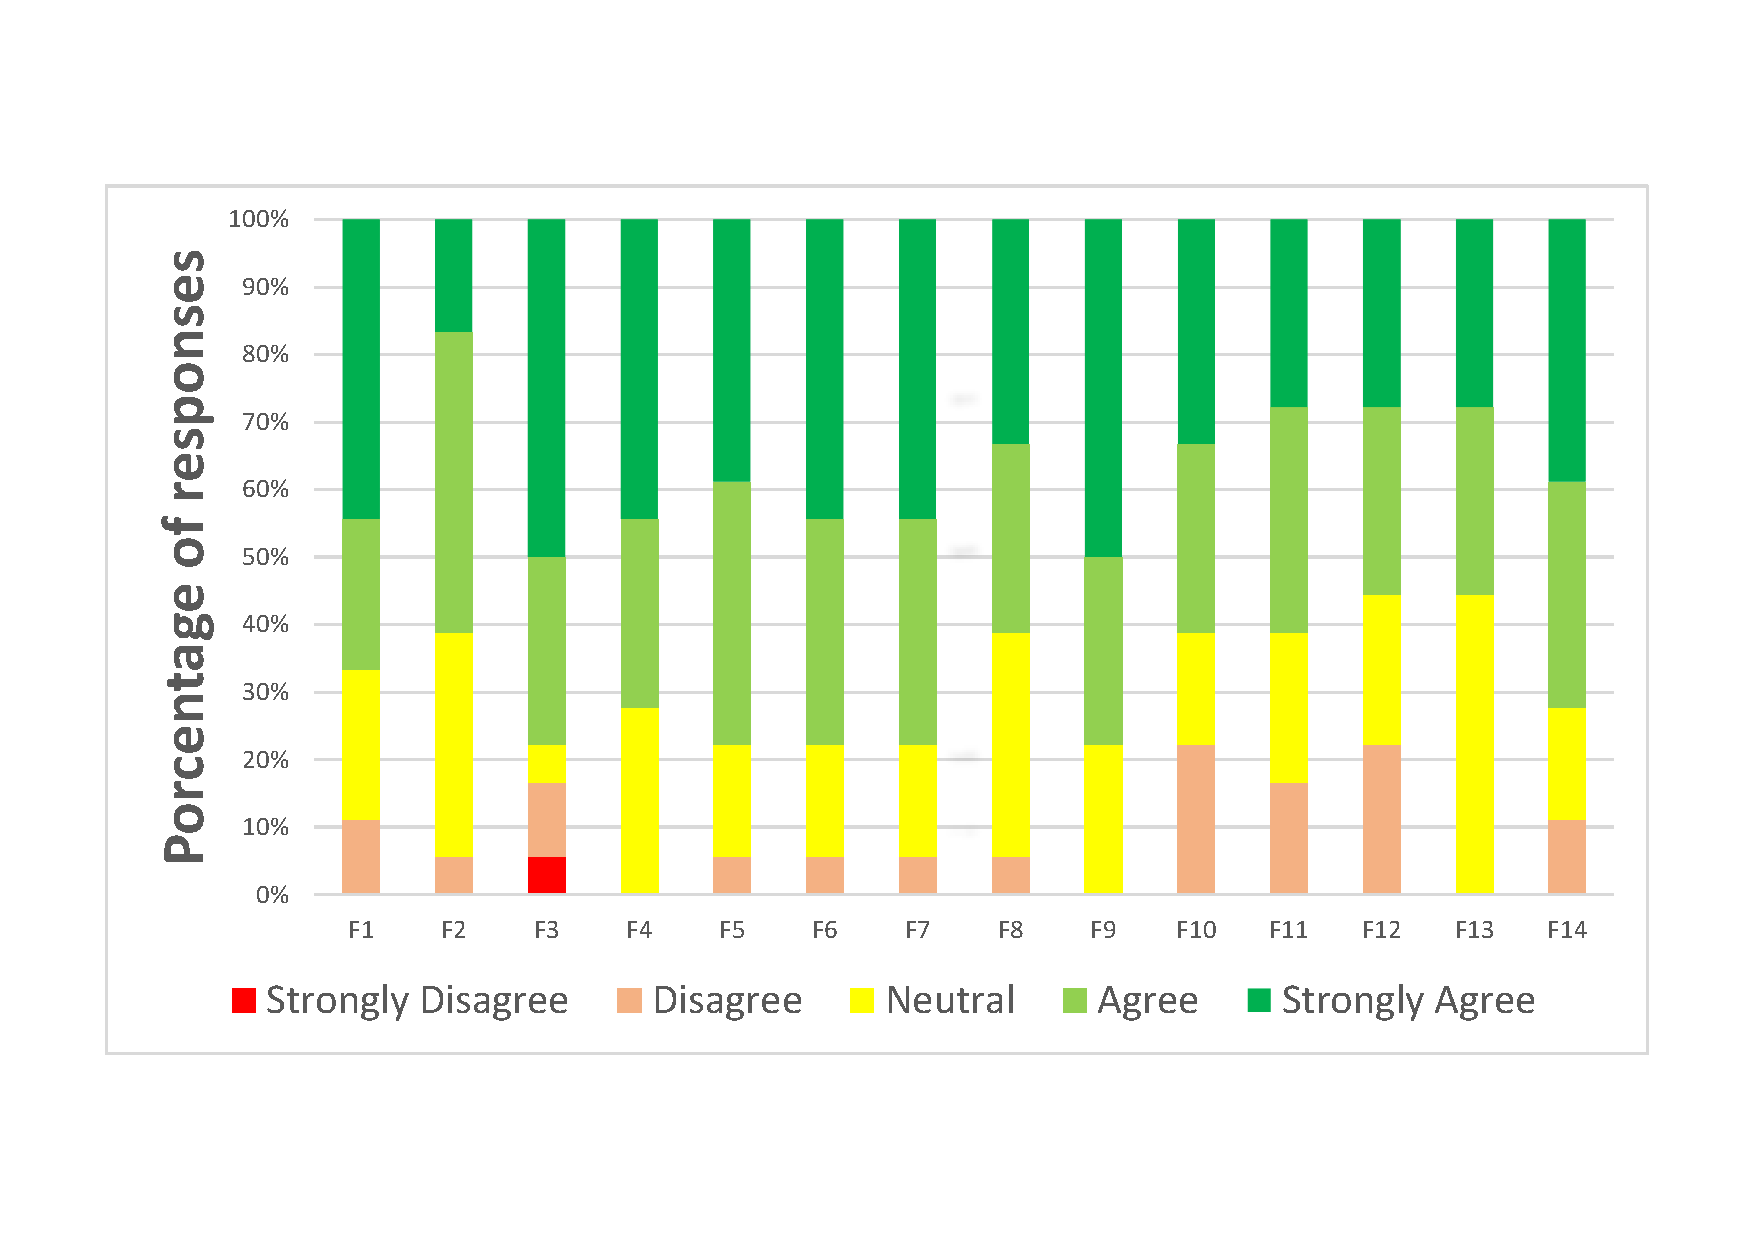
\includegraphics[trim={15mm 25mm 15mm 25mm},clip,width=\linewidth]{IMG/facevalidty.pdf}
    \caption{Gráfica que muestra los porcentajes de respuestas tipo \emph{Likert} en las preguntas de validez aparente.}
    \label{fig:facevalidity}
\end{figure}


\begin{table}[hb]
    \centering
    \begin{tabular}{lp{14cm}}
    \hline
    \multicolumn{2}{c}{Face validity }
    \\
    \hline
    F1:     &  The patient model before selecting the posing is visually realistic.  \\
    F2:     & The deformation of the patient’s internal anatomy is visually realistic.  \\
    F3:     & The previously described steps characterize the procedure in a realistic way.  \\
    F4:     & The placement of the side markers on the x-ray image is visually realistic.   \\
    F5:     & The changes in the final x-ray image due to the adjustment of the beam direction and FRD are visually realistic.  \\
    F6:     & The adjustment of the centre is visually realistic. \\
    F7:     & The changes in the final x-ray image due to the collimation adjustment are visually realistic.  \\
    F8:     & The changes in the final x-ray image due to beam energy configuration are visually realistic.  \\
    F9:     & In general, the changes in the final x-ray image due to modification of the different parameters are visually realistic. \\
    F10:     & The adjustment of the brightness and contrast settings is visually realistic.  \\
    F11:     & The use of image filters is visually realistic.  \\
    F12:     & The simulation of diseases is visually realistic.  \\
    F13:     & The inclusion of foreign objects in the virtual patient is visually realistic.  \\
    F14:     & Generally speaking, the simulator is visually realistic.  \\
    
    \hline
    \end{tabular}
    \caption{Face validity}
    \label{tab:facevalidity}
\end{table}
\clearpage
\subsubsection{Validez de contenido}

Las preguntas relativas a la validez de contenido se pueden leer en la tabla \ref{tab:contentvalidity}. Al igual que el caso anterior, estas preguntas eran de tipo \emph{Likert}, donde se podía responder desde 1(Nada de acuerdo) hasta 5(Muy de acuerdo). 

En la figura \ref{fig:contentvalidity}, se pueden observar los resultados por cada pregunta mostrados en porcentaje de respuestas. Los resultados son parecidos a la validez de apariencia donde se han registrado al menos un 60\% de respuestas positivas en todas las preguntas. 

\begin{figure}[hb]
    \centering
    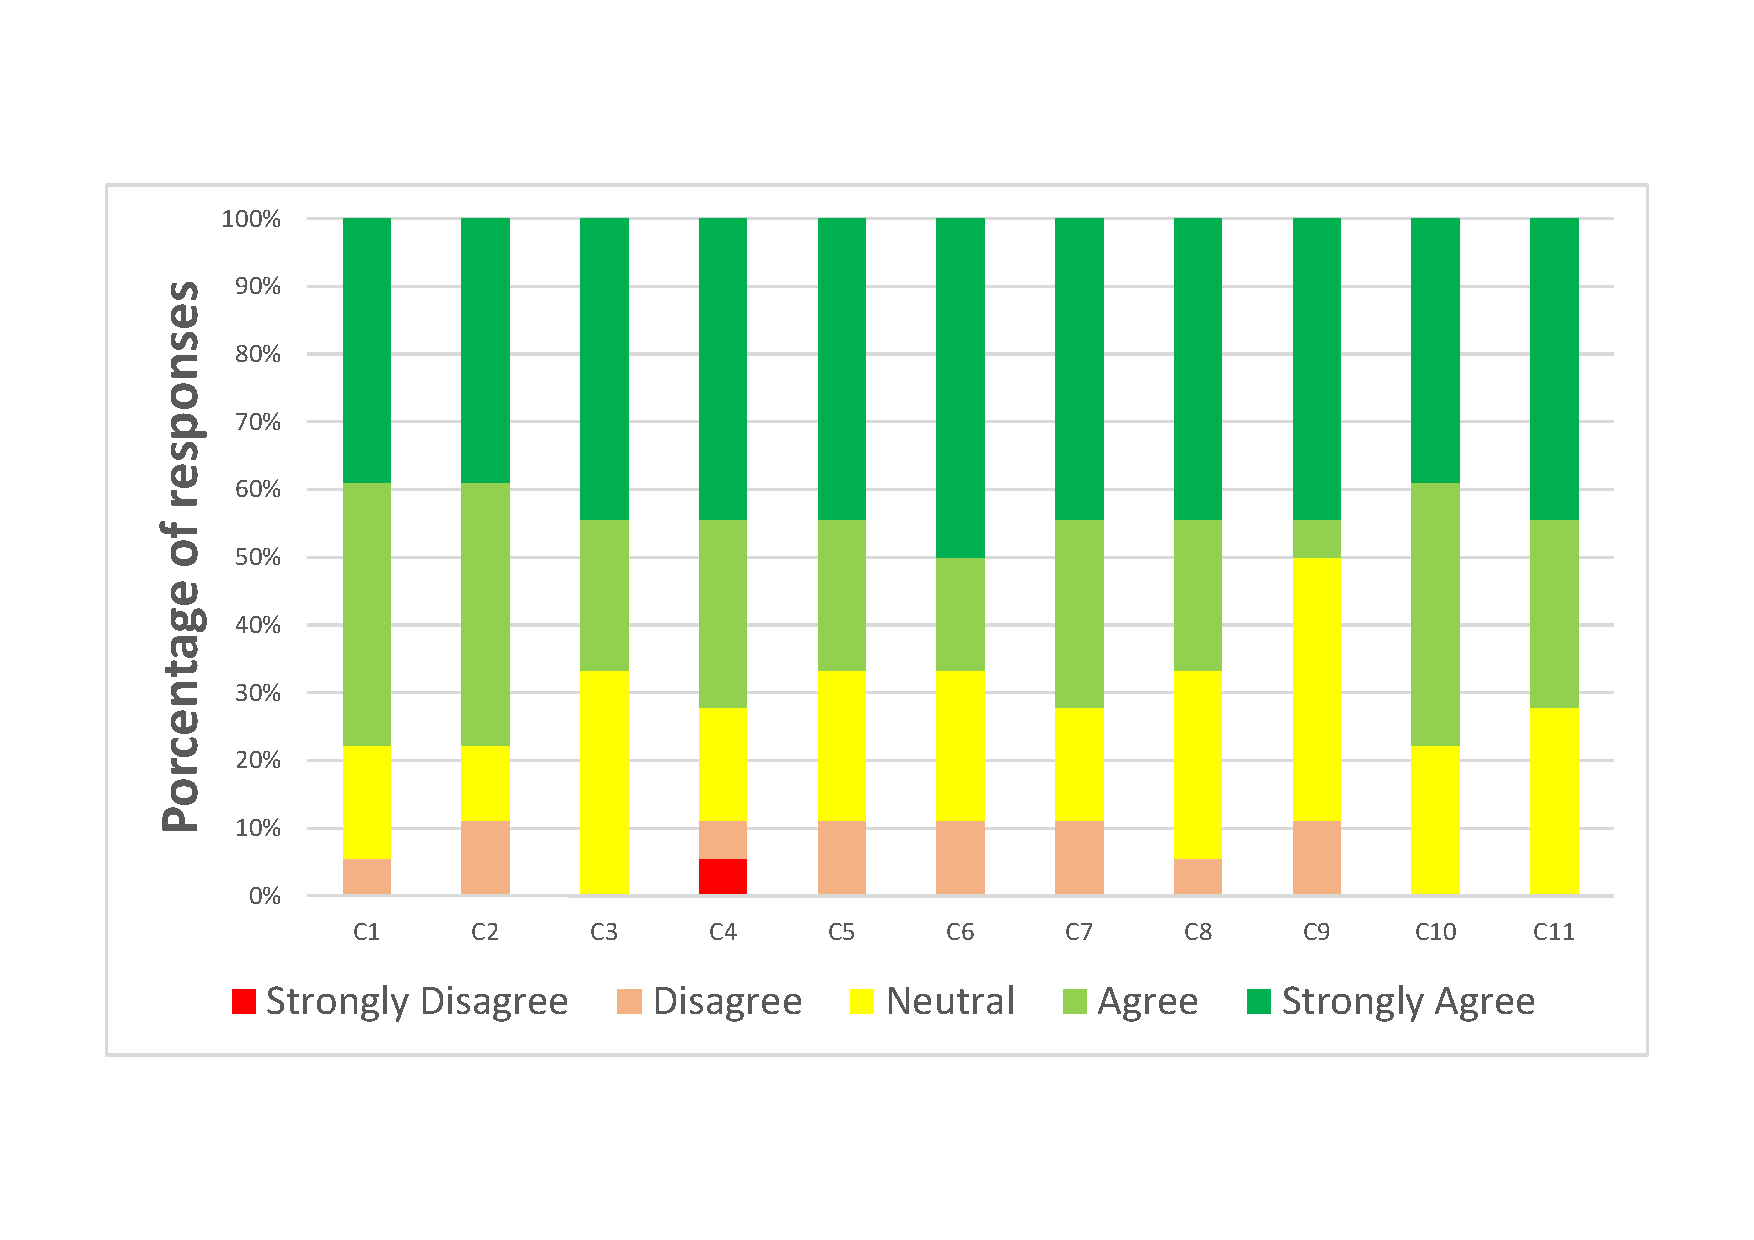
\includegraphics[trim={15mm 25mm 15mm 25mm},clip,width=\linewidth]{IMG/contentvalidty.pdf}
    \caption{Gráfica que muestra los porcentajes de respuestas tipo \emph{Likert} en las preguntas de validez de contenido.}
    \label{fig:contentvalidity}
\end{figure}




\begin{table}[hb]
    \centering
    \begin{tabular}{lp{14cm}}
    \hline
    \multicolumn{2}{c}{Content validity }
    \\
    \hline
    C1:     &  Selecting the patient pose from a set of predefined ones is useful for self-guided training.  \\
    C2:     & Selecting the patient manually is useful for self-guided training.   \\
    C3:     & Selecting the patient pose from a set of predefined ones is useful to teach the procedure.   \\
    C4:     & Selecting the patient manually is useful for teaching purposes (e.g. for live demonstration in the lecture theatre).    \\
    C5:     &  Regarding the previously described steps, the simulator is useful to teach the procedure.  \\
    C6:     & Regarding the previously described steps, the simulator is useful for self-guided training.  \\
    C7:     & In general, digital image manipulation of the X-ray image is useful for self-guided training and teaching.  \\
    C8:     & Regarding the functionality described, this is useful to teach the procedure.   \\
    C9:     & Regarding the functionality described, the simulator is useful  for self-guided training.  \\
    C10:     & Generally speaking, the simulator is suitable is useful as a teaching tool.   \\
    C11:     & Generally speaking, the simulator is suitable for self-guided training.   \\
    \hline
    \end{tabular}
    \caption{Content validity}
    \label{tab:contentvalidity}
\end{table}

Los resultados obtenidos sugieren que el simulador de radiología diagnóstica es visualmente realista. En general, todas las funcionalidades han obtenido una valoración positiva. Además, aunque se registraron pocos comentarios libres, estos comentarios eran positivos. Esto sugiere que, aunque los modelos anatómicos presenten problemas de calidad, a la vista de la mayoría de participantes el simulador proporciona la funcionalidad y el realismo necesario para entrenar el procedimiento. En cuanto a la validez de contenido, las respuestas han sido mayormente positivas, indicando que el simulador es útil para la enseñanza y entrenamiento del procedimiento. 

\clearpage
\subsection{Discusión}
\label{xray:discusion}
Los resultados del simulador muestran una herramienta educativa muy completa que puede ser usada como material complementario para los estudiantes de radiología. La aplicación proporciona un entorno seguro e interactivo para comprobar todo tipo de situaciones. El posicionador de pacientes virtuales permite una interacción en tiempo real con la posibilidad de generar una cantidad de variaciones anatómicas superior a los métodos clásicos como pueden ser los libros o archivos de casos y a los simuladores introducidos en la sección \ref{art:entrenamiento}.

Esta herramienta también demuestra la versatilidad del algoritmo presentado en esta tesis, ya que puede ser incorporado en cualquier simulador que necesite deformaciones plausibles en tiempos interactivos, permitiendo que sea el usuario quien decida la posición final.

Aunque la aplicación se ha diseñado para satisfacer las necesidades de los radiólogos, presenta ciertas limitaciones respecto al procedimiento de diagnóstico por imagen. Existen cuestiones relacionadas con la preparación del paciente para el procedimiento que no pueden ser cubiertas por el simulador, entre ellas las siguientes:

\begin{itemize}
    \item Se recomienda utilizar un lenguaje apropiado y efectivo en la comunicación con los pacientes que no es posible recoger por el simulador.
    \item No se representa la necesidad de indicar al paciente acerca de quitarse prendas u objetos que afecten al área de examen.
    \item No se practican las recomendaciones en cuanto al uso de protectores de plomo para pacientes y profesionales.
    \item Otras comprobaciones que implican condiciones médicas o protocolarias como embarazo, identificación del paciente, etc...
\end{itemize}

Aun así, a la vista de los resultados de las validaciones realizadas, los profesionales han valorado positivamente el simulador. Esto confirma que el simulador puede ser utilizado como herramienta de clase por parte de los profesores, como por el alumnado para practicar el procedimiento. 
